\documentclass[10pt,aspectratio=169]{beamer}

\usepackage[utf8]{inputenc}
\usepackage[T2A]{fontenc}
\usepackage[russian]{babel}

\usepackage{appendixnumberbeamer}
\usepackage{booktabs}
\usepackage{listings}
\usepackage{fontawesome5}
\usepackage{hyperref}
\usepackage{tikz}

\definecolor{primary}{HTML}{1a1a2e}
\definecolor{secondary}{HTML}{16213e}
\definecolor{accent}{HTML}{e94560}
\definecolor{accentlight}{HTML}{fce4ec}
\definecolor{lightbg}{HTML}{f8f9fa}
\definecolor{fg}{HTML}{2d3436}
\definecolor{mgray}{HTML}{636e72}

\setbeamercolor{background canvas}{bg=white}
\setbeamercolor{normal text}{fg=fg}
\setbeamercolor{structure}{fg=primary}

\setbeamercolor{title}{fg=white}
\setbeamercolor{subtitle}{fg=white!70}
\setbeamercolor{author}{fg=white}
\setbeamercolor{institute}{fg=white!60}
\setbeamercolor{date}{fg=white!60}

\setbeamercolor{frametitle}{fg=white,bg=primary}
\setbeamercolor{framesubtitle}{fg=white!70}

\setbeamercolor{block title}{fg=white,bg=primary}
\setbeamercolor{block body}{bg=lightbg}

\setbeamercolor{block title example}{fg=white,bg=secondary}
\setbeamercolor{block body example}{bg=lightbg}

\setbeamercolor{block title alerted}{fg=white,bg=accent}
\setbeamercolor{block body alerted}{bg=accentlight}

\setbeamercolor{section in toc}{fg=fg}
\setbeamercolor{subsection in toc}{fg=mgray}

\setbeamercolor{footline}{fg=white,bg=primary}
\setbeamercolor{page number in head/foot}{fg=white}

\setbeamertemplate{navigation symbols}{}
\setbeamertemplate{footline}{
  \begin{beamercolorbox}[wd=\paperwidth,ht=2.5ex,dp=1ex]{footline}
    \hspace{0.3cm}\textbf{\insertshorttitle}\hfill\textbf{\insertframenumber/\inserttotalframenumber}\hspace{0.3cm}
  \end{beamercolorbox}
}
\setbeamertemplate{frametitle}{
  \begin{beamercolorbox}[wd=\paperwidth,ht=2.8ex,dp=1.2ex]{frametitle}
    \hspace{0.3cm}\textbf{\insertframetitle}
  \end{beamercolorbox}
}

\setbeamertemplate{title page}{
  \begin{tikzpicture}[remember picture,overlay]
    \fill[primary] (current page.north west) rectangle (current page.south east);
    \fill[accent] (current page.north west) rectangle ([xshift=4pt]current page.north east);
  \end{tikzpicture}
  \begin{center}
    \vspace{1.5cm}
    {\usebeamercolor[fg]{title}\Huge\bfseries\inserttitle}\\[0.4cm]
    {\usebeamercolor[fg]{subtitle}\Large\insertsubtitle}\\[1cm]
    \begin{tikzpicture}
      \fill[accent] (0,0) rectangle (4,0.08);
    \end{tikzpicture}\\[0.8cm]
    {\usebeamercolor[fg]{author}\large\insertauthor}\\[0.2cm]
    {\usebeamercolor[fg]{institute}\insertinstitute}\\[0.2cm]
    {\usebeamercolor[fg]{date}\insertdate}
  \end{center}
  \vfill
}

\setbeamertemplate{itemize items}{\color{accent}\faChevronRight}
\setbeamertemplate{enumerate items}[default]
\setbeamercolor{item}{fg=accent}
\setbeamercolor{itemize item}{fg=accent}
\setbeamercolor{itemize subitem}{fg=secondary}

\hypersetup{
  colorlinks=true,
  linkcolor=accent,
  urlcolor=accent
}

\lstset{
  basicstyle=\footnotesize\ttfamily,
  backgroundcolor=\color{lightbg},
  frame=single,
  breaklines=true,
  showstringspaces=false
}

\title{Отказоустойчивый веб-хостинг в VK Cloud}
\subtitle{Итоговый проект --- DevOps/SRE}
\author{Кирилл Ремизов}
\institute{ННГУ им. Лобачевского}
\date{28 июня 2026}

\begin{document}

{
\setbeamercolor{background canvas}{bg=primary}
\begin{frame}[plain]
  \titlepage
\end{frame}
}

\begin{frame}{Содержание}
  \tableofcontents
\end{frame}

\section{Цель проекта}

\begin{frame}{Цель проекта}
  \begin{block}{}
    Развернуть \textbf{отказоустойчивую инфраструктуру} для веб-приложения \\
    (сайт-резюме) в Docker-контейнере на платформе \textbf{VK Cloud}.
  \end{block}

  \vspace{0.4cm}
  \textbf{Ключевые требования:}
  \begin{itemize}
    \item Инфраструктура как код (\texttt{Terraform})
    \item CI/CD через \texttt{GitHub Actions}
    \item Управляемая БД \texttt{PostgreSQL}
    \item Балансировка нагрузки (L7)
    \item Доступность при отказе одного веб-сервера (SLA 99.9\%)
  \end{itemize}
\end{frame}

\section{Выбор варианта}

\begin{frame}{Выбор варианта}
  \textbf{Вариант №1} --- «Отказоустойчивый веб-хостинг на ВМ» \\
  (с заменой ручного Nginx на Docker-контейнер).

  \vspace{0.4cm}
  \textbf{Почему выбран:}
  \begin{itemize}
    \item Покрывает все темы курса: сеть, безопасность, балансировка, БД, автоматизация
    \item Навыки \texttt{Terraform}, \texttt{Docker}, \texttt{CI/CD}, облачные сервисы VK Cloud
    \item Реальный промышленный стек
    \item Чёткие критерии успеха и наглядная демонстрация отказоустойчивости
  \end{itemize}
\end{frame}

\section{Архитектура}

\begin{frame}{Архитектура решения}
  \centering
  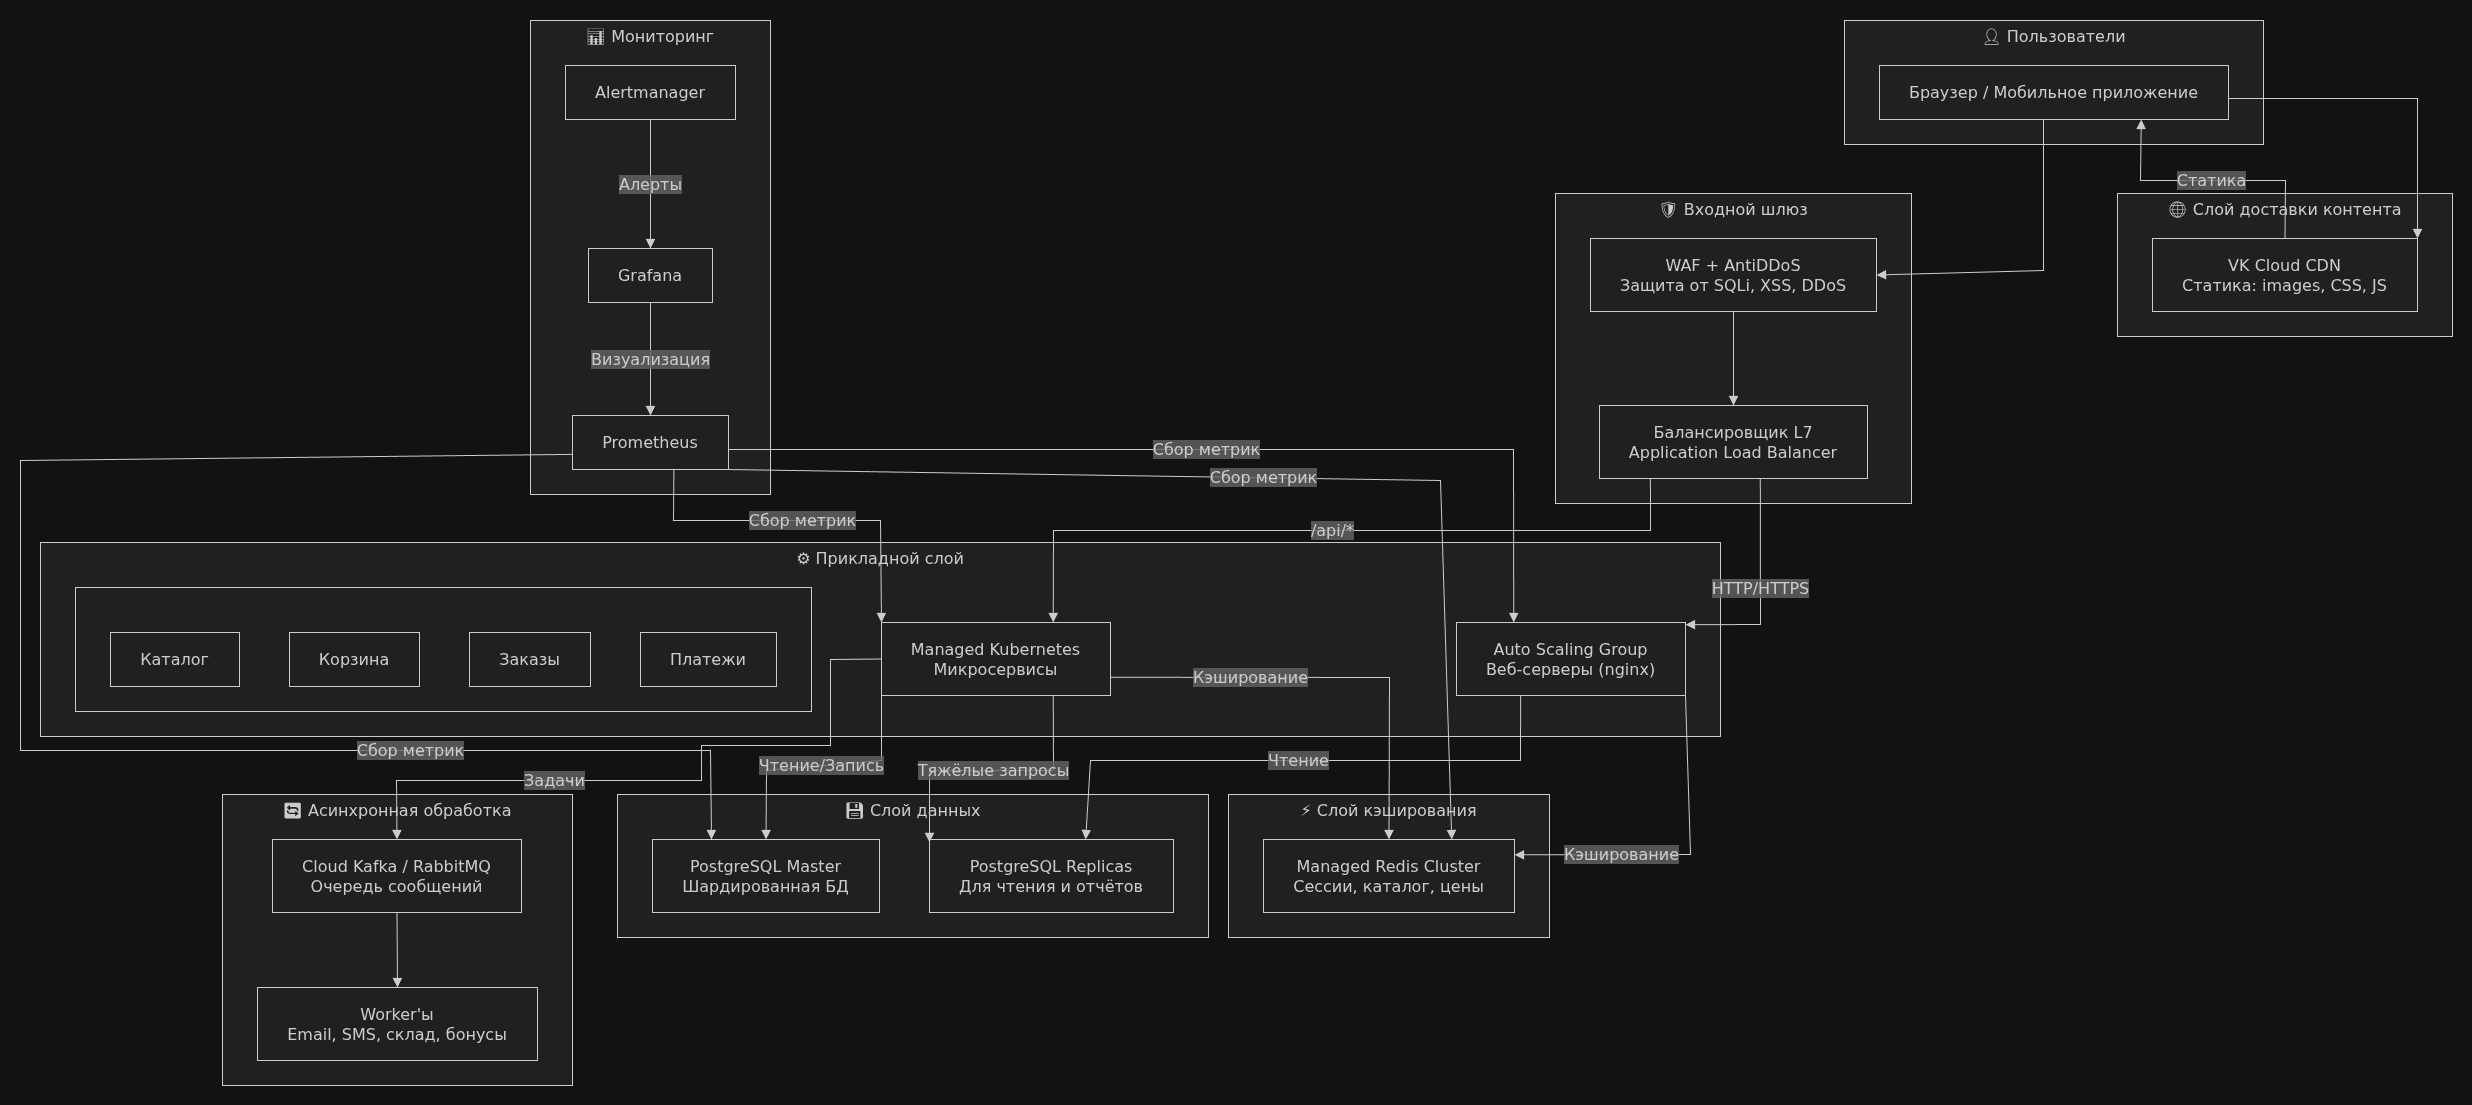
\includegraphics[width=0.82\textwidth]{../exports/VKC_ARCH_M08_highload_store_diogram_РемизовКЛ_20260619.drawio.png}
\end{frame}

\begin{frame}{Компоненты инфраструктуры}

  \begin{columns}[T]
    \begin{column}{0.48\textwidth}
      \textbf{Виртуальные машины}
      \begin{itemize}
        \item 2 веб-сервера (Basic-1-1-10) в приватной подсети
        \item Бастион (Basic-1-1-10) в публичной подсети
      \end{itemize}
      \vspace{0.3cm}
      \textbf{Балансировщик}
      \begin{itemize}
        \item L7 Application Load Balancer
        \item Публичный Floating IP
        \item Health-check: \texttt{GET /DevOps}
        \item Round-robin
      \end{itemize}
    \end{column}
    \begin{column}{0.48\textwidth}
      \textbf{База данных}
      \begin{itemize}
        \item PostgreSQL 14 (Standard-2-8-50)
        \item В приватной подсети
        \item Только изолированный доступ
      \end{itemize}
      \vspace{0.3cm}
      \textbf{Docker}
      \begin{itemize}
        \item Flask + Gunicorn приложение
        \item Образ из приватного реестра
        \item \texttt{--restart=always}
      \end{itemize}
    \end{column}
  \end{columns}
\end{frame}

\begin{frame}{Сеть и безопасность}

  \begin{columns}[T]
    \begin{column}{0.48\textwidth}
      \textbf{VPC / Подсети}
      \begin{itemize}
        \item \texttt{public} (192.168.1.0/24) --- балансировщик + бастион
        \item \texttt{private} (192.168.2.0/24) --- веб-серверы + БД
        \item Internet-шлюз через роутер
      \end{itemize}
    \end{column}
    \begin{column}{0.48\textwidth}
      \textbf{Security Groups}
      \begin{itemize}
        \item \texttt{main}: HTTP (80) для всех, SSH (22) только с моего IP
        \item \texttt{db\_sg}: PostgreSQL (5432) только из приватной подсети
        \item Доступ к веб-серверам --- только через бастион
      \end{itemize}
    \end{column}
  \end{columns}

  \vspace{0.5cm}
  \begin{alertblock}{}
    \centering
    Единственная точка входа --- бастион с Floating IP, \\
    SSH разрешён только с IP автора
  \end{alertblock}
\end{frame}

\section{Стек технологий}

\begin{frame}{Стек технологий}
  \centering
  \begin{tabular}{ll}
    \toprule
    \textbf{Компонент} & \textbf{Технология} \\
    \midrule
    Инфраструктура & \texttt{Terraform} (provider vkcs) \\
    Оркестрация & \texttt{Docker} (контейнеры на ВМ) \\
    Балансировка & VK Cloud Load Balancer (L7) \\
    База данных & VK Cloud DBaaS (PostgreSQL 14) \\
    CI/CD & GitHub Actions \\
    Хранение состояния & S3 (VK Cloud Object Storage) \\
    Приложение & Python (Flask) + Gunicorn \\
    \bottomrule
  \end{tabular}

  \vspace{0.4cm}
  \texttt{Rust}, \texttt{C++}, \texttt{Linux}, \texttt{Bash} --- доп. компетенции
\end{frame}

\section{Terraform}

\begin{frame}{Terraform --- инфраструктура как код}

  Terraform-конфигурация разбита на 4 файла:

  \begin{itemize}
    \item \texttt{main.tf} --- провайдеры, сеть, ВМ, балансировщик, БД
    \item \texttt{variables.tf} --- все переменные с умолчаниями
    \item \texttt{outputs.tf} --- выходные данные (IP, параметры БД)
    \item \texttt{backend.tf} --- S3 backend для хранения state
  \end{itemize}

  \vspace{0.3cm}
  \begin{block}{Ключевые ресурсы}
    \texttt{vkcs\_compute\_instance.web[count=2]} --- 2 веб-сервера \\
    \texttt{vkcs\_lb\_loadbalancer} --- L7 балансировщик \\
    \texttt{vkcs\_db\_instance.postgres} --- управляемая PostgreSQL \\
    \texttt{vkcs\_compute\_instance.bastion} --- бастион-хост
  \end{block}
\end{frame}

\begin{frame}[fragile]{Terraform --- user\_data веб-сервера}

  \begin{lstlisting}
#!/bin/bash
apt-get update
apt-get install -y docker.io
systemctl enable docker
systemctl start docker
sleep 5
docker run -d --restart=always \
  -p 80:80 ${var.docker_image}
  \end{lstlisting}

  \vspace{0.3cm}
  \begin{itemize}
    \item Автоматическая установка Docker при создании ВМ
    \item Pull из приватного реестра (до 5 повторных попыток)
    \item \texttt{--restart=always} --- автоматический перезапуск
  \end{itemize}
\end{frame}

\section{CI/CD}

\begin{frame}{GitHub Actions --- CI/CD Pipeline}

  \begin{columns}[T]
    \begin{column}{0.48\textwidth}
      \textbf{Jobs:}
      \begin{enumerate}
        \item \textbf{Plan} --- инициализация, валидация, план
        \item \textbf{Apply} --- применение (только push в main)
        \item \textbf{Destroy} --- удаление инфраструктуры
      \end{enumerate}
    \end{column}
    \begin{column}{0.48\textwidth}
      \textbf{Secrets:}
      \begin{itemize}
        \item \texttt{VKCS\_USERNAME}
        \item \texttt{VKCS\_PASSWORD}
        \item \texttt{VKCS\_PROJECT\_ID}
        \item \texttt{SSH\_PUBLIC\_KEY}
        \item \texttt{S3\_ACCESS/SECRET\_KEY}
      \end{itemize}
    \end{column}
  \end{columns}

  \vspace{0.3cm}
  \begin{exampleblock}{}
    \centering
    \faGithub ~ Push в main $\rightarrow$ автоматический деплой инфраструктуры
  \end{exampleblock}
\end{frame}

\section{Проверка}

\begin{frame}{Проверка работоспособности}

  \begin{enumerate}
    \item Просмотр ресурсов в консоли VK Cloud
    \item Доступность сайта через браузер \\
          \hfill\url{http://95.163.213.173/DevOps}
    \item SSH через бастион к веб-серверам, \texttt{docker ps}
    \item \textbf{Отказоустойчивость:} \texttt{docker stop} на web-1 \\
          \hfill$\rightarrow$ сайт продолжает работать
    \item Запуск контейнера обратно, возврат в пул
    \item Подключение к PostgreSQL через \texttt{psql}
    \item Нагрузочное тестирование \texttt{ab}
  \end{enumerate}
\end{frame}

\begin{frame}{Результаты нагрузочного тестирования}

  \centering
  \texttt{ab -n 1000 -c 10 http://95.163.213.173/DevOps}

  \vspace{0.3cm}
  \begin{tabular}{lr}
    \toprule
    \textbf{Параметр} & \textbf{Значение} \\
    \midrule
   Полных запросов & 1000 \\
   Ошибок & 1 (Length) \\
   Запросов/сек & 76.54 \\
   Время на запрос (mean) & 130.65 мс \\
   Transfer rate & 816.36 КБ/с \\
   95\% перцентиль & 113 мс \\
    \bottomrule
  \end{tabular}

  \vspace{0.3cm}
  \begin{exampleblock}{\centering 99.9\% успешных запросов --- цель достигнута}
  \end{exampleblock}
\end{frame}

\section{Результаты}

\begin{frame}{Результаты проекта}

  \begin{columns}[T]
    \begin{column}{0.48\textwidth}
      \textbf{Выполнено:}
      \begin{itemize}
        \item Отказоустойчивая инфраструктура в VK Cloud
        \item Fully automated CI/CD (GitHub Actions)
        \item Infrastructure as Code (Terraform)
        \item Docker-контейнеризация приложения
        \item L7 балансировка + Health-check
        \item Управляемая PostgreSQL
        \item Нагрузочное тестирование
      \end{itemize}
    \end{column}
    \begin{column}{0.48\textwidth}
      \textbf{Задел на будущее:}
      \begin{itemize}
        \item Пароль БД в коде (Vault)
        \item Health-check по \texttt{/DevOps} (не \texttt{/health})
        \item Образ с тегом \texttt{latest}
        \item Нет мониторинга (Prometheus/Grafana)
        \item Нет автообновления контейнеров
      \end{itemize}
    \end{column}
  \end{columns}
\end{frame}

\begin{frame}{Репозитории проекта}

  \centering
  \vspace{0.3cm}
  \begin{block}{\faGithub ~ GitHub (основной)}
    \centering
    \url{https://github.com/BlackCorbeau/final_assessment}
  \end{block}

  \vspace{0.2cm}
  \begin{block}{\faGitAlt ~ Forgejo (зеркало)}
    \centering
    \url{https://git.rustprogersteam.ru/Black_Raven/MyResume}
  \end{block}

  \vspace{0.5cm}
  \begin{center}
    \textbf{\Huge\color{accent}?}
  \end{center}
\end{frame}

\end{document}
